\documentclass{article}
\usepackage{amsmath,amssymb,amsfonts}  % For math symbols and fonts
\usepackage{graphicx}                   % For including images
\usepackage{hyperref}                   % For hyperlinks
\usepackage{cite}                       % For citations

\usepackage{algorithm}
\usepackage{algorithmic}

\usepackage{amsthm}
% Define new theorem-like environments
% Define environments
\theoremstyle{definition} % Non-italicized style
\newtheorem{definition}{Definition}[section]
\newtheorem{exercise}{Exercise}[section]

% Title and author info
\title{Makes drones in cirle Experiments Report}
\author{Zhang Jinrui\thanks{alternative email:zhangjr1022@mails.jlu.edu.cn} \\ \texttt{jerryzhang40@gmail.com}}

\date{20250720}  % Empty date; optional, you can also specify a date here

\begin{document}

\maketitle

\begin{abstract}
    In this article, I tried to do apply a
    simple policy to each drone to make
    them fly in cirle
\end{abstract}

\section{recite of the problem \& assumptions}
There are 10 drones and fly on the sky
obeys Newton's second law of motion.
which is
\[
    \vec{F} = m \vec{a}
\]
\[
    \vec{a} = \frac{d\vec{v}}{dt} = \frac{d^2 \vec{x}}{dt^2}
\]
And I mean the policy by, we need a function of force
depending on some communication between drones
to decide the \(\vec{F}\)
\[
    \vec{F}=f(the current information)
\]

And then we want the following dynamic system
\[\begin{bmatrix}
        \frac{d\vec{d}}{dt} \\
        \frac{d\vec{v}}{dt}
    \end{bmatrix}=
    \begin{bmatrix}
        \vec{v} \\
        \vec{a}=f/m
    \end{bmatrix}
\]
has some Self-organized emergent phenomena,
to automatically emergent a circle rounding pattern.

\section{a simple prompt}
To be more clear of the notations we use,
we have \(i\in\{1,2,...,10\}=N\)
And the drones are ignored of its flying
height, which the position vector can be a
2d vector note it as \(\vec{d_i}\)
And so the velocity and acceleration we denote as
\(\vec{v_i}=\frac{d\vec{d_i}}{dt}\)
and
\(\vec{a_i}=\frac{d\vec{v_i}}{dt}\)
I want to prompt a \(f\) so that it can form
a cirle.
\[
    \vec{f_i}=m_i(\sum_{\forall k\neq i,\|\vec{d_i}-\vec{d_k}\|\leq R}(\frac{\vec{d_i}-\vec{d_k}}{\|\vec{d_i}-\vec{d_k}\|^3})+(\frac{\vec{d_{t(i)}}-\vec{d_i}}{\|\vec{d_{t(i)}}-\vec{d_i}\|}-v_i))
\]
This model is easy to explain, the first term is
just a inverse square propell force, the second
term is make the velocity quickly approch a set direction
the \(t(i)\) is just a randomly choosed target drone
other than \(i\) that is \(t(i)\in N, t(i)\neq i\)

This formula can be rewrite without physical term as
follow.
\[
    \vec{a_i}=\sum_{\forall k\neq i,\|\vec{d_i}-\vec{d_k}\|\leq R}(\frac{\vec{d_i}-\vec{d_k}}{\|\vec{d_i}-\vec{d_k}\|^3})+(\frac{\vec{d_{t(i)}}-\vec{d_i}}{\|\vec{d_{t(i)}}-\vec{d_i}\|}-v_i)
\]
separately view this is combined by two independent force
\[
    (\vec{a_i})_{target}=(\frac{\vec{d_{t(i)}}-\vec{d_i}}{\|\vec{d_{t(i)}}-\vec{d_i}\|}-v_i)
\]
\[
    (\vec{a_i})_{propell}=\sum_{\forall k\neq i,\|\vec{d_i}-\vec{d_k}\|\leq R}(\frac{\vec{d_i}-\vec{d_k}}{\|\vec{d_i}-\vec{d_k}\|^3})
\]

\section{a simple prompt:simulation}
\subsection{Four drone case}
\subsubsection{derivation}
This case just choose \(N=\{1,2,3,4\}\)
and don't allow \(t(t(i))=i\)
which definitely form a three element loop and
a dangling drone.

We have a (4,2)-tensor \(\vec{d_i}\)
and two other (4,2)-tensor \(\vec{v_i}\)
and \(\vec{a_i}\)
The initial points are randomly choosed
in Uniformly \([0,1]\times[0,1]\)

choose a time increment \(dt\)
and the simulation update formula is simple to write

just as follow
\[\begin{bmatrix}
        \vec{{d_{n+1}}_i} \\
        \vec{{v_{n+1}}_i}
    \end{bmatrix}=
    \begin{bmatrix}
        \vec{{d_{n}}_i}+\vec{{v_n}_i}dt \\
        \vec{{v_{n}}_i}+(\sum_{\forall k\neq i,\|\vec{{d_n}_i}-\vec{{d_n}_k}\|\leq R}(\frac{\vec{{d_n}_i}-\vec{{d_n}_k}}{\|\vec{{d_n}_i}-\vec{{d_n}_k}\|^3})+(\frac{\vec{{d_n}_{t(i)}}-\vec{{d_n}_i}}{\|\vec{{d_n}_{t(i)}}-\vec{{d_n}_i}\|}-{v_n}_i))dt
    \end{bmatrix}
\]

simple Euler method.
\subsubsection{code \& result}
the computational code are \cite[Euler-Maruyama]{HEAT-EM} and \cite[PDE]{HEAT-PDE}.
the results are shown by the following pictrues which
generated by the code.
I have done some normalization to make the scale of
the PDE solution same as the Euler-Maruyama solution.
\begin{figure}[ht!]
    \centering
    \begin{minipage}{0.45\textwidth}
        \centering
        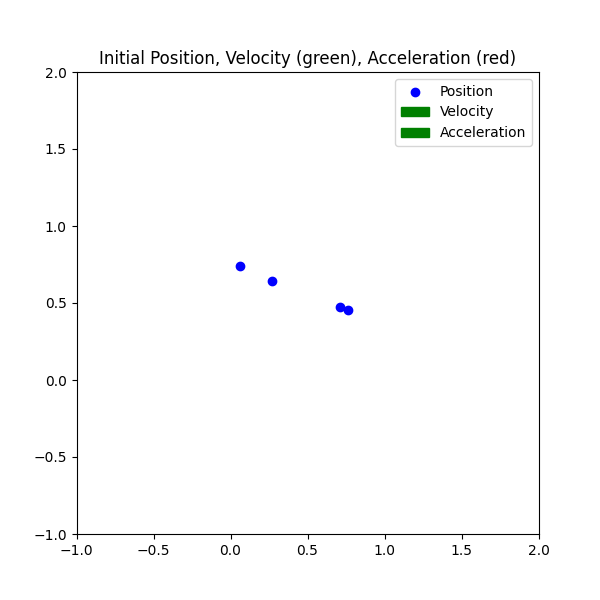
\includegraphics[width=0.9\textwidth]{fig/sample1/dd.png} % first figure itself
        \caption{Euler-Maruyama method}
        \label{fig:fig4}
    \end{minipage}\hfill
    \begin{minipage}{0.45\textwidth}
        \centering
        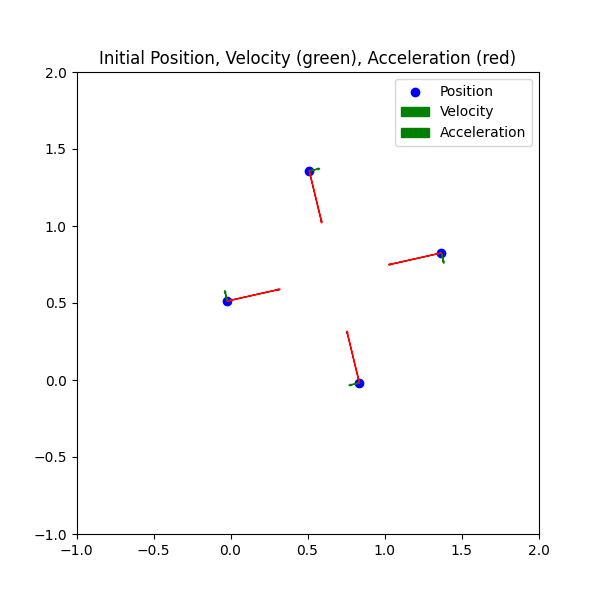
\includegraphics[width=0.9\textwidth]{fig/sample1/dd_18254.png} % second figure itself
        \caption{PDE method}
    \end{minipage}
\end{figure}

\section{some analysis why it will have a stability property}
\subsection{the terminate radius R}
undergoing
\subsection{the terminate center O}
undergoing
\subsection{graph theory part}
The \(t(i)\) forms a graph which have \(n\) points
and \(n\) oriented edges, this forms a tree with a extra
edges, and this case It will obviously form a Unicyclic Graph.

Which is a tree if we treat all the point on the
loop as the same point.


\section{PDE and Euler-Maruyama:roadmap}
the current roadmap contains three separate comparison.
basically I want to do same comparison over three
equations.
\[
    \dot{\mathbf{X}} =  \nabla U(\mathbf{X}) +  \,\epsilon\boldsymbol{\eta}(t)
\]
\[
    \dot{\mathbf{X}} =  \epsilon\boldsymbol{\eta}(t)
\]
and
\[
    \dot{\mathbf{X}} =  \nabla U(\mathbf{X})
\]
These three equations can be written in their
PDE form according to
\cite[Fokker-Planck Equation]{Fokker-Planck}
as follow.
\[
    \frac{\partial p}{\partial t} =  \frac{\epsilon^2}{2}  \Delta p\,-\nabla\cdot(p\nabla U)
\]
\[
    \frac{\partial p}{\partial t} = \frac{\epsilon^2}{2}  \Delta p
\]
and
\[
    \frac{\partial p}{\partial t} =  -\nabla\cdot(p\nabla U)
\]

For each equation, I'll use both PDE solver
to get the \(p(x,t)\).and the Euler-Maruyama method
to sample paths and get the distribution

\section{PDE and Euler-Maruyama:experiments}
\subsection{simulation of the heat equation}
\subsubsection{PDE part}
The equation will have a form of the following,
if we only care about the wenier term.
\[
    \dot{\mathbf{X}} =  \epsilon\boldsymbol{\eta}(t)
\]
if we consider the probabilistic distribution function
over time. We have.
\[
    \frac{\partial p}{\partial t} = \frac{\epsilon^2}{2}  \Delta p
\]
This is a heat equaiton.

To make this one feasible for computer to
deal with I constrain the space interver
just in \(X=(0,0.1)\), and time period in
\(T=(0,1)\).

So I need to add a boundary condition.
For a heat equation, which from a brownian
motion I think choose the derivative free condition
is fit this case which is,
\[
    \frac{\partial p}{\partial x}(x,t) = 0 , x\in\partial X, t\in T
\]
and a initial distribution I choose the following
function,
\[
    p(x,0)=\frac{-1}{1 + e^{-100 * (x - 0.9)}}+\frac{1}{(1 + e^{-100 * (x - 0.1)})}
\]
Although this is not a normalized distribution,
but it's okay for the simulation i think.


\subsubsection{Euler-Maruyama part}
We have a second method which is the
Euler-Maruyama method which we sample
the initial value through distribution
\(p(x,0)\) and do the Euler-Maruyama
method to get a lot solution
\(x_k(t)\) then the distribution of
\(x_k(t)\) should be equation to
\(p(x,t)\)

the iteration relation as following
\[
    x_{n+1}=x_n+\sqrt{\Delta t}\,\xi_n,\xi_n\sim \mathcal{N}(0, 1)
\]

\subsubsection{code \& results}
the computational code are \cite[Euler-Maruyama]{HEAT-EM} and \cite[PDE]{HEAT-PDE}.
the results are shown by the following pictrues which
generated by the code.
I have done some normalization to make the scale of
the PDE solution same as the Euler-Maruyama solution.
% \begin{figure}[ht!]
%     \centering
%     \begin{minipage}{0.45\textwidth}
%         \centering
%         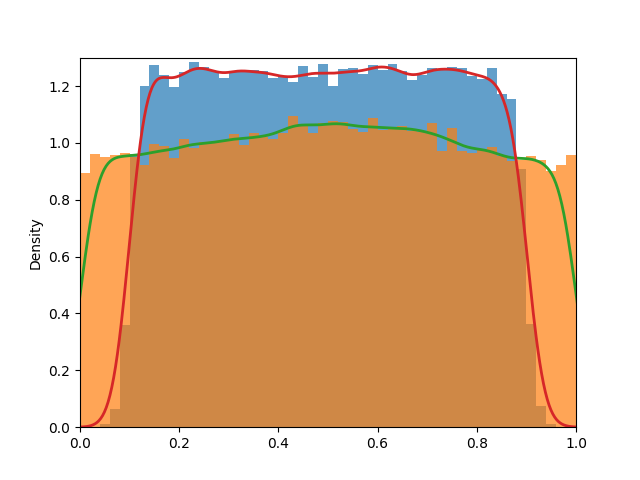
\includegraphics[width=0.9\textwidth]{fig/distributioncombine.png} % first figure itself
%         \caption{Euler-Maruyama method}
%         \label{fig:fig4}
%     \end{minipage}\hfill
%     \begin{minipage}{0.45\textwidth}
%         \centering
%         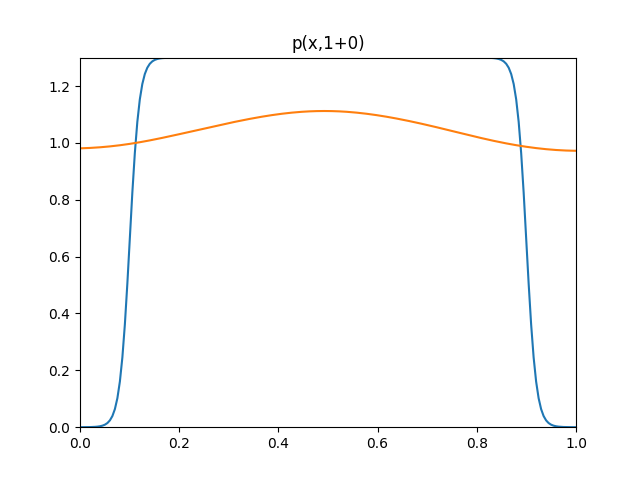
\includegraphics[width=0.9\textwidth]{fig/p(x,1+0).png} % second figure itself
%         \caption{PDE method}
%     \end{minipage}
% \end{figure}

\subsection{simulation of definite equation}
\subsubsection{PDE part}
undergoing.
\subsubsection{Euler-Maruyama part}
undergoing.
\subsection{simulation of the combined equation}
\subsubsection{PDE part}
undergoing.
\subsubsection{Euler-Maruyama part}
undergoing.

\section{roadmap}
The main idea to solve this equation is
to use the pinn\cite{raissi2017physics} to fitting the solution
distribution \(p(x,t)\)
where for every \(t\) we have
\(\int_{-\infty}^{\infty}p(x,t)dx=1\)

We need a differential equation about this
\(p(x,t)\) to make the pinn work.

First we need to find a differential
relation only involves \(p(x,t)\).
Then we can use pinn to get the solution
distribution \(p(x,t)\).

\subsection{definite equation}
To simplify the original equation
\[
    \dot{\mathbf{X}} =  \nabla U(\mathbf{X}) +  \,\boldsymbol{\eta}(t)
\]
We first remove the wenier term,
as following.
\[
    \dot{\mathbf{X}} =  \nabla U(\mathbf{X})=u
\]

For a short period of time increment \(dt\)
the problem involves two distribution
\(p(x,t)\) and \(p(x,t+dt)\)
and we choose a initial point at \(t\)
denote as \(x_t\) and the solution point
at time \(t+dt\) is \(x_{t+dt}\)

So the Lagrangian derivative
is as follow
\[
    \frac{Dp}{Dt} = \frac{\partial p}{\partial t} + u \cdot \nabla p
\]
\[
    \frac{Dp}{Dt}=\frac{p(x_{t+dt},t+dt)-p(x_{t},t)}{dt}
\]
and Consider the probabilistic mass around the
point \(x_{t+dt}\) and \(x_{t}\) we can get a following
relation
\[p(x_{t+dt},t+dt)(dx)(e^{vdt})=p(x_{t},t)(dx)\],
where \[v=\nabla \cdot u\]
which is the same as follow
\[p(x_{t+dt},t+dt)=p(x_{t},t)(e^{-vdt})\]
as the \(dt\) is infinitesimal so
\(e^{-vdt}=1-vdt\)
so we can get
\[
    p(x_{t+dt},t+dt)-p(x_{t},t)=-vdt
\]
which is
\[
    \frac{Dp}{Dt}=-v=-\nabla \cdot u=-\Delta U=\frac{\partial p}{\partial t} + u \cdot \nabla p
\]
then we get a formula only involves \(p(x,t)\)
\[
    \frac{\partial p}{\partial t} + u \cdot \nabla p +\nabla \cdot u=0
\]
the initial distribution may take any thing,
but for one case we can chose the dirac function
\[
    p(x,0)=\delta(x - x_0)
\]
in this case this model is just a plain
ODE. but in a distribution case.

\subsection{sochastic equation}
Add back the wenier term the equation backs to
\[
    \dot{\mathbf{X}} =  \nabla U(\mathbf{X}) +  \,\boldsymbol{\eta}(t)
\]
For the same period of time increment \(dt\)
the problem involves two distribution
\(p(x,t)\) and \(p(x,t+dt)\)
and we choose a initial point at \(t\)
denote as \(x_t\) and the solution point
at time \(t+dt\) is \(x_{t+dt}\)

then for the point relations by the solution of the
equation, \(x_t\) gose to \(x_{t+dt}\)
we denote this as \(x_{t+dt}=F(x_t)\)
and \(x_{t}=B(x_{t+dt})\)

For a certain point \(x\) at time \(t+dt\)
we want \(p(x,t+dt)\)
this involves a convolution process.
\[
    p(x,t+dt)=\int_{-\infty}^{\infty}g(y)p(B(x),t)e^{-vdt}dy
\]
where $g(y)$ is the probabilistic density function of
normal distribution
\[
    \mathcal{N}(0, dt)
\]
If we can some how transform this equation to a
differential equation only involves
\(p(x,t)\), then we can solve this
by pinn as the definite model.
But this process is way too hard to deal.

\subsection{sochastic equation:sampling}
I suppose to sample the
\[
    \boldsymbol{\eta}(t)
\]
According to the time discrete size when we
use pinn.
when we have sample a specific sample of
\[
    \boldsymbol{\eta}_k(t)
\]
we can then rewrite
\[
    \dot{\mathbf{X}} =  u_t=\nabla U(\mathbf{X}) +  \,\boldsymbol{\eta}_k(t)
\]
\[
    \frac{\partial p}{\partial t} + u_t \cdot \nabla p +\nabla \cdot u_t=0
\]
sove this equaiton we can get a sample solution
\[
    p_k(x,t)
\]
to sample a lot
\[
    \boldsymbol{\eta}_k(t)
\]
we can average all the \(p_k\)
to get the estimated distribution function
\(p\sim\frac{\sum_{k=1}^{N}p_k}{N}\)











\bibliographystyle{plain}  % or another style like unsrt, IEEEtran, etc.
\bibliography{references}  % references.bib is the file name

\end{document}
